\section[\textit{Slew Limiters}]{\textit{Slew Limiters}}
\sectionmark{\textit{Slew Limiters}}
\label{sec:slew_limiters}

Un \textit{Slew Limiter}, también conocido como \textit{rate limiter}, limita la velocidad de cambio de una señal y, por tanto, su pendiente. Su efecto es el de suavizar la señal al redondear sus cambios bruscos. Cuando una señal de entrada tiene componentes frecuenciales mayores a la del \textit{Slew limiter}, estas son eliminadas en la señal de salida. Synthi 100 posee tres de estos módulos, cuya único parámetro, controlable por voltaje, es la <<tasa de cambio>> (fig. \ref{fig:slew_limiters}). 

\begin{figure}
	\centering
	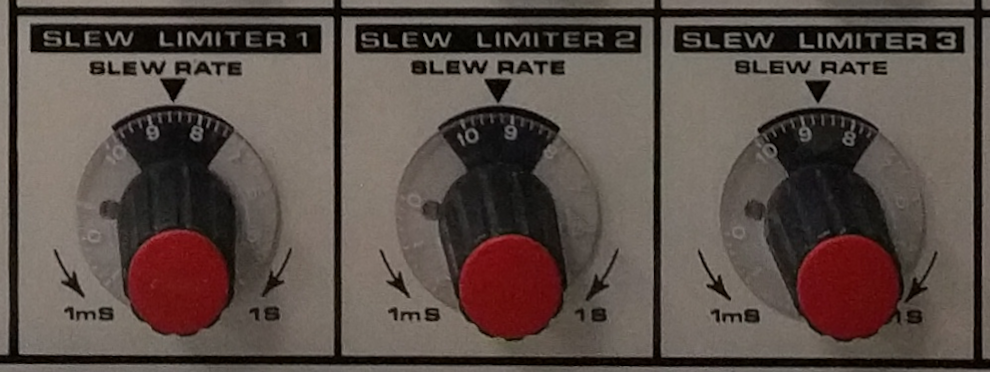
\includegraphics[width=0.7\textwidth]{images/slew_limiters}
	\caption[\textit{Slew Limiters}]{Los tres \textit{Slew Limiters} del Synthi 100 del GME.}
	\label{fig:slew_limiters}
\end{figure}

\subsection{Implementación en \appName}
Existen varios \textit{UGens} que pueden de variar la <<tasa de cambio>> de una señal de entrada, si bien solo uno, \texttt{Slew}, está optimizado hacerlo con una de audio. El resto (\texttt{Var}, \texttt{Var2}, \texttt{VarLag} o \texttt{LagUD}) están más recomendados para las señales de control. La implementación del \texttt{Synth} es totalmente trivial debido a que los parámetros de \texttt{Slew} coinciden con los del Synthi 100. 